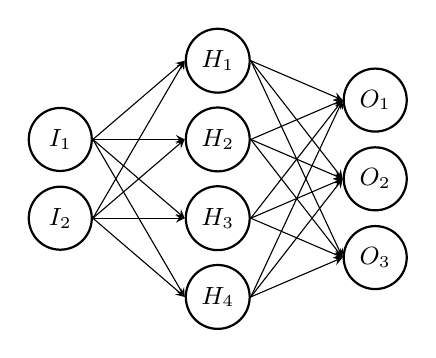
\begin{tikzpicture}[>=stealth, ->, 
  node distance=1.5cm,
  every node/.style={circle, draw, 
  minimum size=0.8cm, font=\small, thick}]

% Couche d'entrée (2 neurones)
\node (I1) at (0, 0.5) {$I_1$};
\node (I2) at (0,-0.5) {$I_2$};

% Couche cachée (4 neurones)
\node (H1) at (2,1.5) {$H_1$};
\node (H2) at (2,0.5)  {$H_2$};
\node (H3) at (2,-0.5) {$H_3$};
\node (H4) at (2,-1.5) {$H_4$};

% Couche de sortie (3 neurones)
\node (O1) at (4,1) {$O_1$};
\node (O2) at (4,0)  {$O_2$};
\node (O3) at (4,-1) {$O_3$};

% Connexions : Entrée -> Cachée
\foreach \i in {1,2}
  \foreach \j in {1,2,3,4}
    \draw (I\i.east) -- (H\j.west);

% Connexions : Cachée -> Sortie
\foreach \j in {1,2,3,4}
  \foreach \k in {1,2,3}
    \draw (H\j.east) -- (O\k.west);

\end{tikzpicture}
